\documentclass[12pt,compress,aspectratio=169]{beamer}

\usetheme{metropolis}
\setbeamersize{text margin left=.5cm,text margin right=.5cm}
\setbeamertemplate{navigation symbols}{} % suppress nav bar
%\setbeamercovered{transparent}

\usefonttheme{professionalfonts}
\usepackage{amsmath,bm}
\usepackage{siunitx}
\usepackage{tikz}
\usepackage{mathpazo}
%\usepackage[scaled]{helvet}
\usepackage{xcolor,colortbl}

\setsansfont{Roboto Light}
\setmonofont{Ubuntu Mono}
\setlength{\parskip}{0pt}
\renewcommand{\baselinestretch}{1}

\sisetup{
  detect-all,
  math-sf=\textsf,
  number-math-rm=\mathnormal,
  per-mode=symbol
}

\usetikzlibrary{decorations.pathmorphing,patterns}


\title{Topic 3: Work and Energy}
\subtitle{Advanced Placement Physics 1}
\author[TML]{Dr.\ Timothy Leung}
\institute{Olympiads School}
\date{\today}


\newcommand{\pic}[2]{\includegraphics[width=#1\textwidth]{#2}}
\newcommand{\mb}[1]{\ensuremath\mathbf{#1}}
\newcommand{\kkk}{\ensuremath\hat{\bm{k}}}
\newcommand{\eq}[2]{\vspace{#1}{\Large\begin{displaymath}#2\end{displaymath}}}

\begin{document}

\begin{frame}
  \maketitle
\end{frame}

\begin{frame}{Files for You to Download}
  These are the slides and homework questions for this week.
  \begin{itemize}
  \item\texttt{PhysAP1-03-workEnergy.pdf}--Slides on work and energy
  \item\texttt{PhysAP1-04-momentum.pdf}--Slides on momentum, impulse and
    general collisions
  %\item\texttt{PhysAP1-03-Homework.pdf}--Homework problems for this topic.
  \end{itemize}
  Please download/print the PDF file before class. There is no advantage to
  copying notes that are already printed out for you. Instead, focus on details
  that aren't necessarily on the slides. If you want to print the slides, we
  recommend that you print 4 slides per page to save paper.
\end{frame}



\begin{frame}{Work and Energy}
  We start with some definition at are (unfortunately) not very useful:
  \begin{itemize}
    \item \textbf{Energy} is the ability to do work.
    \item \textbf{Work} is the mechanism in which energy is transformed.
  \end{itemize}
  Luckily, we can also use equations to define these concepts.
\end{frame}


\section{Work}

\begin{frame}{Mechanical Work}
  \textbf{Mechanical work} is performed when a force $\mb{F}$ displaces an
  object by $\Delta \mb{x}$. If the force is \emph{constant}, then the work
  done is given by the dot product between the force and displacement vectors:

  \eq{-.2in}{
    \boxed{W=\mb{F}\cdot\Delta\mb{x}}
    \quad\text{\normalsize or}\quad
    \boxed{W=|\mb{F}||\mb{\Delta x}|\cos\theta}
  }

  \vspace{-.15in}where $\theta$ is the angle between the two vectors. When
  force and displacement vectors are expressed by the IJK notation, work is:

  \eq{-.2in}{
    W=F_x\Delta x+F_y\Delta y+F_z\Delta z
  }

  From the definition of a dot product
\end{frame}

\begin{frame}{Mechanical Work}

  Mechanical work is a scalar quantity:
  
  \eq{-.2in}{
    \boxed{W=\mb{F}\cdot\Delta\mb{x}}
  }
  
%  is applied to move an object from $\mb{x}_1$ to $\mb{x}_2$ along a path, then
%  the total work done by the force is defined by the integral:
%
%  \eq{-.2in}{
%    W=\int\mb{F}(\mb{x})\cdot d\mb{x}
%  }
  \begin{itemize}
  \item No work done if no displacement ($\Delta\mb{x}=\mb{0}$)
  \item No work done when $\mb{F}\perp\Delta\mb{x}$, when (i.e.\
    $\mb{F}\cdot\Delta\mb{x}=0$; the force did not cause the displacement)
  \item Work can be positive or negative depending on the dot product (or in
    the scalar case, $\cos\theta$)
%  \item When there are multiple forces acting on an object, we can c1ompute the
%    work done by each \emph{each} force
  \end{itemize}
\end{frame}



%\begin{frame}{Work by Non-Constant Force}
%  For a non-constant force, there are a few ways to deal with the problem:
%  %if the object moves along straight path, the integral
%  simplifies to just the dot product of the two vectors:
%
%
%  Or in the scalar form that is more familiar in Grades 11/12 Physics that
%  avoid vector notations:
%
%  \eq{-.2in}{

%  }
%\end{frame}



\begin{frame}{Definition of Mechanical Work}
  \textbf{Work done by a force}
  \begin{itemize}
  \item The work done by \emph{one specific force}
  \item Example: A boy pushes a cart forward. The ``work done by the boy'' is
    the work done by the applied force.
  \end{itemize}

  \vspace{.15in}\textbf{Work done on an object}
  \begin{itemize}
  \item There may be more than one force acting on an object
  \item The \emph{sum} of all the work done on the object by each force
  \item The work done by the net force
  \item Also called the \textbf{net work} $W_\mathrm{net}$
  \end{itemize}
\end{frame}



\section{Kinetic Energy}

\begin{frame}{Kinetic Energy}
  When a constant net force accelerates an object from $v_0$ to $v_1$, work is
  being done (can be positive or negative). Combining a kinematic equation with
  the second law of motion:

  \eq{-.2in}{
      v_1^2 =v_0^2+2\textcolor{red}{a}\Delta x =
      v_0^2+2\textcolor{red}{\frac{F_\mathrm{net}}{m}}\Delta x
  }

  Re-arranging terms and solving for $F_\mathrm{net}\Delta x$ (the work done by
  $F_\mathrm{net}$), we get a familiar expression:

  \eq{-.2in}{
    F_\mathrm{net}\Delta x = \frac{1}{2}m(v_1^2-v_0^2)
    =\frac{1}{2}mv_1^2- \frac{1}{2}mv_0^2
  }
  

  
%  When a net force on an object accelerates it, the resulting amount of
%  work done on the object (net work $W_{\textrm{net}}$) is given by:
%
%  \eq{-.2in}{
%    W_{\textrm{net}}=\int\mb{F}_{\textrm{net}}\cdot d\mb{x}=\int m\mb{a}\cdot d\mb{x}
%    =m\int\frac{d\mb{v}}{dt}\cdot d\mb{x}
%  }
%
%  Since both $\mb{v}$ and $\mb{x}$ are continuous functions in
%  time, we can switch the order of differentiation, i.e.:
%
%  \eq{-.2in}{
%    =m\int\frac{d\mb{x}}{dt}\cdot d\mb{v}=m\int\mb{v}\cdot d\mb{v}
%    =m\int_{v_1}^{v_2} vdv %=\Delta\left(\frac{1}{2}mv^2\right)=\Delta K
%  }
%
%  and since $\mb{v}$ and $d\mb{v}$ must be in the same direction, the dot
%  product is trivial: $\mb{v}\cdot d\mb{v}=vdv$
\end{frame}



\begin{frame}{Kinetic Energy}
  The change in the ``quantity of motion'' caused by the work done is defined
  as the \textbf{translational kinetic energy} $K$:

  \eq{-.1in}{
    \boxed{K=\frac12mv^2}
  }

  Later in the course we will discuss \emph{rotational} kinetic energy.
  We arrive at this result using calculus even when $F_\mathrm{net}$ is not
  constant.
\end{frame}



\begin{frame}{Work and Kinetic Energy}
  %In fact, the \emph{definition} of kinetic energy came from this integration,
  %in that work equals to the change in \emph{something}, and we define that as
  %kinetic energy.
  The \textbf{work-energy theorem} states that:

  \eq{-.15in}{
    \boxed{W_\mathrm{net}=\Delta K}
  }

  We don't have to prove this theorem because kinetic energy is defined to
  fit this theorem.
  \begin{itemize}
  \item $\Delta K$ can be positive or negative depending on whether the work
    done is positive or negative
  \item When multiple forces acting on an object, each force can add/remove
    kinetic energy from an object
  \end{itemize}
\end{frame}



%\begin{frame}{Example}
%  \textbf{Example 1:} A force $\mb{F}=4.0x\bm{\hat{\imath}}$ (in newtons) acts
%  on an object of mass \SI{2.}{\kilo\gram} as it moves from $x=1.0$ to
%  $x=\SI{5.}{\metre}$. Given that the object is at rest at $x=1$,
%  \begin{enumerate}[(a)]
%  \item Calculate the net work
%  \item What is the final speed of the object?
%  \end{enumerate}
%\end{frame}



\section{Potential Energy}

\begin{frame}{Gravitational Force \& Gravitational Potential Energy}
  The gravitational force (weight) of an object is defined as:
  
  \eq{-.25in}{
    \mb{w}=m\mb{g}
  }
  
  \vspace{-.1in}Near Earth's surface, $\mb{g}=-g\kkk$ can be considered to be
  constant. Using the definition of mechanical work, the work done to move an
  object from height $h_0$ to $h_1$ is therefore:

  \eq{-.2in}{
    W=\mb{w}\cdot\Delta\mb{h}
    =-mg\kkk\cdot\Delta h\kkk
    =-\left[mgh_1-mgh_0\right]%=-\Delta U_g
  }

  From this, we define the \textbf{gravitational potential energy} $U_g$:

  \eq{-.2in}{
    U_g=mgh
  }
\end{frame}




\begin{frame}{Spring Force \& Elastic Potential Energy}
  The spring force $\mb{F}_e$ is the force that a compressed/stretched spring
  exerts on the object connected to it. It obeys Hooke's law:
    
  \eq{-.2in}{
    \mb{F}_e=-k\mb{x}
  }

  \vspace{-.1in}We can find the work done to displace a spring using some
  calculus that is not shown here:

  \eq{-.3in}{
    W=\mb{F}_e\cdot\Delta\mb{x}=\frac12kx_1^2-\frac12kx_0^2
  }
  
  From this we define the \textbf{elastic potential energy} $U_e$:

  \eq{-.2in}{
    U_e=\frac12kx^2
  }
\end{frame}



\begin{frame}{Conservative Forces}
  Gravitational force, spring force, electrostatic force (studied in Grade 12
  Physics) are called \textbf{conservative forces}
  \begin{itemize}
  \item The work done by these forces relate to a change of another quantity
    called \emph{potential energy}
  \item Since the potential energy is evaluated at the end points, the work
    done by a conservative force is \emph{path independent}
  \end{itemize}
\end{frame}



\begin{frame}{Conservative Forces}
  With a little bit of calculus, a constant conservative forces can be related
  to the change in potential energy by the expression in one-dimension:
%  Expressions for potential energies are obtained by integrating the work done
%  by the conservative forces, these forces are therefore the negative gradient
%  of the potential energies:
%
%  \eq{-.2in}{
%    \mb{F}=-\nabla U=
%    -\frac{\partial U}{\partial x}\bm{\hat{\imath}}
%    -\frac{\partial U}{\partial y}\bm{\hat{\jmath}}
%    -\frac{\partial U}{\partial z}\hat{\bm{k}}
%  }
%
%  The direction of a conservative force \emph{always} decreases the potential
%  energy. In 1D:

  \eq{-.2in}{
    \boxed{
      F=-\frac{\Delta U}{\Delta x}
    }
  }

  Pay attention to the negative sign. Students often forget it.
\end{frame}




\begin{frame}{Work and Potential Energy}
  With conservative forces, \emph{in addition} to changing kinetic energy,
  work equals to the change in \emph{something}, and we define that
  as \emph{potential energy}. Therefore:

  \eq{-.2in}{
    W_{\textrm{cons.}}=-\Delta U
  }
  \begin{itemize}
  \item\vspace{-.15in}$\Delta U$ can be positive/negative depending on the
    direction of the conservative force
  \item Positive work \emph{decreases} potential energy, while
  \item Negative work \emph{increases} potential energy
  \end{itemize}
\end{frame}



\begin{frame}{Conservation of Mechanical Energy}
  Positive work done by conservative forces on an object does two things:
  \begin{enumerate}[1.]
  \item\emph{Decrease} its potential energy, while
  \item\emph{Increase} its kinetic energy by the same amount
  \end{enumerate}
  In other words:

  \eq{-.25in}{
    W_\mathrm{cons.}=-\Delta U = \Delta K
  }

  \vspace{-.15in}This means that total mechanical energy $E$ must be conserved
  when only conservative forces are doing work, or that the total \emph{change}
  in mechanical energy is zero:
  
  \eq{-.2in}{
    \boxed{\Delta E=\Delta K + \Delta U =0}
  }

  \vspace{-.15in}That's why those forces are called conservative forces!
\end{frame}



\section{Conservation of Energy}

%\begin{frame}{Isolated Systems and the Conservation of Energy}
%  An \textbf{isolated system} is a system of objects that does not interact with
%  the surrounding. Think of an isolated system as a bunch of objects inside an
%  insulated box.
%  \begin{center}
%    \begin{tikzpicture}[scale=.8]
%      \fill[pattern=north east lines] (0,0) rectangle(5,4);
%      \draw[ultra thick] (0,0) rectangle(5,4);
%      \draw[ultra thick,fill=white](.25,.25) rectangle(4.75,3.75);
%      \draw[thick,
%        decoration={aspect=.3,segment length=2mm, amplitude=2.5mm, coil},
%        decorate] (2.5,3.75)--(2.5,2.25) node[midway,right]{$\;\;k$};
%      \draw[fill=black!40](2,2.25) rectangle(3,1.25) node[midway]{$m$};
%    \end{tikzpicture}
%  \end{center}
%\end{frame}
%
%
%\begin{frame}{Isolated Systems and Conservation of Energy}
%  \begin{itemize}
%  \item Since the system is isolated from the surrounding environment, the
%    environment can't do any work on it, by definition!
%  \item Likewise, the energy inside the system cannot escape either
%  \item Therefore energy of the system is conserved
%  \item There are \emph{internal} force inside the system that is doing work,
%    but the work only converts kinetic energy into potential energies, and vice
%    versa.
%  \end{itemize}
%\end{frame}



\begin{frame}{Example: Horizontal Spring-Mass System}
  Total mechanical energy is conserved when there are only conservative forces.
  \begin{itemize}
  \item Assuming that there is no friction in any part of the system
  \item The isolated system consists of the mass and the spring
  \end{itemize}  
  Energies:
  \begin{itemize}
  \item Kinetic energy of the mass
  \item Elastic potential energy stored in the spring
  \end{itemize}
  \begin{center}
    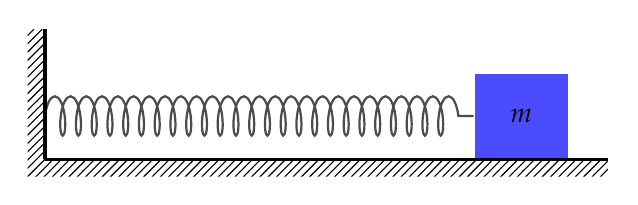
\begin{tikzpicture}[scale=1.1]
      \node[fill=blue!70,inner sep=4.5mm] (a) at (5.5,1) {$m$};
      \draw[thick,draw=black!70,
        decoration={aspect=.3,segment length=2mm, amplitude=2.5mm, coil},
        decorate] (0,1)--(4.95,1);
      \fill [pattern=north east lines] (6.5,.5)--(6.5,.3)--(-.2,.3)
      --(-.2,2)--(0,2)--(0,.5)--cycle;
      \draw[very thick] (0,.5)--(6.5,.5);
      \draw[very thick] (0,.5)--(0,2);
    \end{tikzpicture}
  \end{center}
\end{frame}


\begin{frame}{Example: Gravity}
  Gravity is another example, as an object falls towards Earth's surface,
  the only force acting on it is its weight, which is conservative:
  \begin{center}
    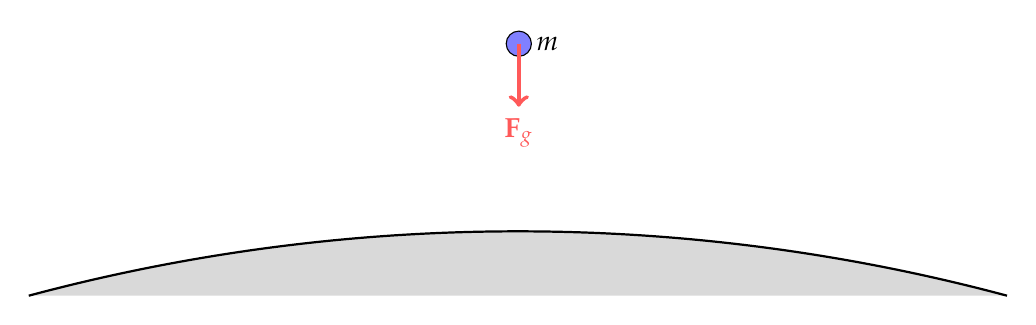
\begin{tikzpicture}[scale=.8]
      \draw[thick,fill=gray!30] (7.75,0) arc(75:105:30);
      \draw[fill=blue!50] (0,4) circle(.2) node[right]{$\;m$};
      \draw[ultra thick, red!65,->] (0,4)--(0,3) node[pos=1,below]{$\mb{F}_g$};
    \end{tikzpicture}
  \end{center}
  Assuming no friction, the total mechanical energy consists of:
  \begin{itemize}
  \item Kinetic energy of the mass
  \item Gravitational potential energy of the mass
  \end{itemize}
\end{frame}



\begin{frame}{Example: Vertical spring-mass system}
  \begin{columns}
    \column{.2\textwidth}
    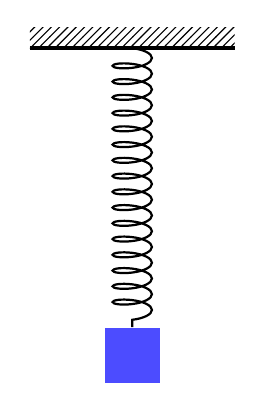
\begin{tikzpicture}[scale=1.3]
      \node[fill=blue!70,inner sep=3.5mm] (b) at (1,2) {};
      \draw[thick,
        decoration={aspect=.3,segment length=2mm, amplitude=2.5mm, coil},
        decorate] (1,5)--(b); 
      \fill [pattern=north east lines] (0,5) rectangle (2,5.2);
      \draw[ultra thick] (0,5)--(2,5);
    \end{tikzpicture}

    \column{.8\textwidth}
    In a vertical spring-mass system, the work done on the mass are the
    spring force and gravity (both are conservative). Therefore the energy
    stored in the system are:
    \begin{itemize}
    \item Kinetic energy of the mass
    \item Gravitational potential energy of the mass
    \item Elastic potential energy stored in the spring
    \end{itemize}
    The total mechanical energy of the system is conserved if there is no
    friction
  \end{columns}
\end{frame}


\begin{frame}{What if there is friction?}
  Energy is always conserved as long as your system is defined properly
  \begin{columns}
    \column{.2\textwidth}
    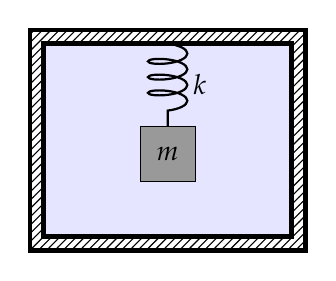
\begin{tikzpicture}[scale=.7]
      \fill[pattern=north east lines] (0,0) rectangle(5,4);
      \draw[ultra thick] (0,0) rectangle(5,4);
      \draw[ultra thick,fill=blue!10](.25,.25) rectangle(4.75,3.75);
      \draw[thick,
        decoration={aspect=.3,segment length=2mm, amplitude=2.5mm, coil},
        decorate] (2.5,3.75)--(2.5,2.25) node[midway,right]{$\;\;k$};
      \draw[fill=black!40](2,2.25) rectangle(3,1.25) node[midway]{$m$};
    \end{tikzpicture}
    \column{.8\textwidth}
    \begin{itemize}
    \item The system consists of a mass, a spring, Earth and all the air
      particles inside the box
    \item As the mass vibrates, friction with air slows it down
    \item While the mass loses energy, the temperature of the air rises due to
      friction
    \item Energies:
      \begin{itemize}
      \item Kinetic and gravitational potential energies of the mass
      \item Elastic potential energy stored in the spring
      \item Kinetic energy of the vibration of the air molecules
      \end{itemize}
    \item Total energy is conserved even as the mass stops moving
    \end{itemize}
  \end{columns}
\end{frame}



\begin{frame}{Conservation of Energy}
  If \emph{only} conservative forces do work, then the total mechanical energy
  (sum of all the kinetic and potential $K+U$ energies) is conserved:

  \eq{-.1in}{
    \boxed{\sum K_i +\sum U_i =\sum K_i'+\sum U_i'}
  }

  (The summation notation is used because there can be multiple particles,
  each with its kinetic energy, and multiple potential energies being stored).
  This is consistent with the equation shown in the previous slide:

  \eq{-.2in}{
    \boxed{\Delta E=\Delta K + \Delta U =0}
  }
\end{frame}



\begin{frame}{Conservation of Energy}
  When non-conservative forces are also doing work, the work done by those
  forces $W_{\textrm{nc}}$ must be taken into account as well:
%  instead of
%  \emph{trying} to isolate the system, we can calculate the work done by them
%  $W_{\textrm{nc}}$ and add it to the total energy of the system
    
  \eq{-.2in}{
    \boxed{\sum K_i +\sum U_i +\sum W_{\textrm{nc}}=\sum K_i'+\sum U_i'}
  }

  Expressed in terms the total mechanical energy (like in the previous slides),
  the conservation of energy equation becomes:
  
  \eq{-.2in}{
    \boxed{\Delta E=\sum\Delta K_i + \sum\Delta U_i =W_\mathrm{net}}
  }

  We do not have to distinguish between conservative and non-conservative work
  in this equation (only non-conservative work contributes to $\Delta E$).
\end{frame}



\begin{frame}{Non-Conservative Force}
  Work done by these non-conservative forces are \emph{usually} negative
  because they oppose the direction of motion
  \begin{itemize}
  \item Drag (fluid resistance)
  \item Kinetic friction
  \end{itemize}
  The work done by these non-conservative forces may be positive or negative,
  depending on the problem
  \begin{itemize}
  \item Applied force
  \item Tension force
  \item Normal force
  \end{itemize}
  Note that the work-kinetic energy theorem still applies when non-conservative
  forces are present
\end{frame}


\begin{frame}{Example}
  \textbf{Example 2:} A mass $m$ is dropped from a height of $h$ above the
  equilibrium position of a spring. Set up the equation that determines the
  spring's compression $d$ when the object is instantaneously at rest.
  \begin{center}
    \pic{.35}{spring-example1.png}
  \end{center}
\end{frame}


%\begin{frame}{Example}
%  \textbf{Example 3:} A mass $m$ is pulled a distance $d$ up an incline (angle
%  of elevation $\theta$) at constant speed using a rope that is parallel to
%  the incline. The coefficient of friction is $\mu_k$.
%  \begin{enumerate}[(a)]
%  \item What is the magnitude of the tension force in the rope?
%  \item What is the magnitude of the normal force?
%  \item What is the work done by the normal force?
%  \item What is the work done by friction?
%  \item What is the work done by the tension force?
%  \item What is the net work?
%  \item What is the change in total mechanical energy?
%  \item Show that $\Delta E_\mathrm{mech}=W_\mathrm{non-conservative}$.
%  \end{enumerate}
%\end{frame}


%\begin{frame}{Energy Diagrams}
%  \begin{itemize}
%  \item Plots of potential energy ($U$) vs.\ position for a conservative force
%    \begin{center}
%      \pic{.5}{energy-diagram.png}
%    \end{center}
%  \item If more than one conservative force, they can be combined into one graph
%  \item Where slope is zero means no force acting on it: it is in a state of
%    \textbf{equilibrium}
%  \item An object placed at an equilibrium point with $K=0$ will remain there
%  \end{itemize}
%\end{frame}



\section{Power \& Efficiency}

\begin{frame}{Power}
  \textbf{Power} is the \emph{rate} at which work is done, i.e.\ the rate at
  which energy is being transformed. The average power $\overline{P}$ is work
  done over a finite time interval $\delta t$. The unit for power is a
  \textbf{watt} \si{\watt}:

  \eq{-.15in}{
    \boxed{\overline{P} = \frac{W}{\Delta t}}
  }
  \begin{center}
    \begin{tabular}{l|c|c}
      \rowcolor{pink}
      \textbf{Quantity}  & \textbf{Symbol} & \textbf{SI Unit} \\ \hline
      Average power  & $\overline{P}$ & \si{\watt} \\
      Work done      & $W$            & \si{\joule} \\
      Time interval  & $\Delta t$     & \si{\second}
    \end{tabular}
  \end{center}
  In engineering, power is often more critical than the actual amount of work
  done.
\end{frame}



\begin{frame}{Power}
  If a constant force is used to push an object at a constant velocity, the
  power produced by the force is:
  
  \eq{-.1in}{
    P=\frac{W}{\Delta t}=\frac{\mb{F}\cdot\Delta\mb{x}}{\Delta t}
    =\mb{F}\cdot\frac{\Delta\mb{x}}{\Delta t}
    \quad\rightarrow\quad
    \boxed{P=\mb{F}\cdot\mb{v}}
  }
  
  Application: aerodynamics
  \begin{itemize}
  \item When an object moves through air, the applied force must overcome air
    resistance (drag force), which is proportional with $v^2$
    \item Therefore ``aerodynamic power'' must scale with $v^3$ (i.e.\ doubling
      your speed requires $2^3=8$ times more power)
    \item Important when aerodynamic forces dominate
  \end{itemize}
\end{frame}



\begin{frame}{Efficiency}
  \textbf{Efficiency} is the ratio of useful energy or work output to the total
  energy or work input

  \eq{-.2in}{
    \boxed{\eta = \frac{E_o}{E_i}\times\SI{100}{\percent}}\quad
    \boxed{\eta = \frac{W_o}{W_i}\times\SI{100}{\percent}}
  }
  \begin{center}
    \begin{tabular}{l|c|c}
      \rowcolor{pink}
      \textbf{Quantity} & \textbf{Symbol} & \textbf{SI Unit} \\ \hline
      Useful output energy & $E_o$ & \si{\joule} \\
      Input energy         & $E_i$ & \si{\joule} \\
      Useful output work   & $W_o$ & \si{\joule} \\
      Input work           & $W_i$ & \si{\joule} \\
      Efficiency           & $\eta$ & no units
    \end{tabular}
  \end{center}
  Efficiency is always $0\leq\eta\leq\SI{100}{\percent}$
\end{frame}
\end{document}
